% 第 18 题四棱锥 P-ABCD：顶点坐标按固定源 PDF 矢量路径端点换算（1 pt → 0.04 cm）。
% 实线 6 段：AD（一线段，E 在其中点）、EP、DP、CD、CP、AP；虚线 6 段：CE、AB、BE、BC、BD、BP。
% 全图唯一相交处：虚线 CE 与实线 DP（虚线在交点两侧断开、实线连续）——先画虚线后画实线即得。
% PA 竖直；BC ∥ AD（同高）且 BC = AD/2（投影保持）；E 为 AD 中点。
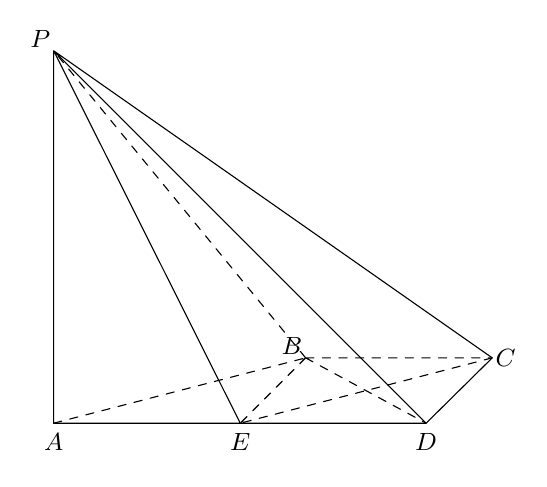
\begin{tikzpicture}[line cap=round,line join=round,font=\small]
\coordinate (P) at (-2.80,4.90);
\coordinate (A) at (-2.80,0.17);
\coordinate (E) at (-0.43,0.17);
\coordinate (D) at (1.93,0.17);
\coordinate (B) at (0.40,1.00);
\coordinate (C) at (2.77,1.00);
% 虚线先画
\draw[dashed] (C)--(E) (A)--(B) (B)--(E) (B)--(C) (B)--(D) (B)--(P);
% 实线后画（压住虚线交叉处，与原图一致）
\draw (A)--(D) (E)--(P) (D)--(P) (C)--(D) (C)--(P) (A)--(P);
\node[above left,inner sep=1pt] at (P) {$P$};
\node[below] at (A) {$A$};
\node[below] at (E) {$E$};
\node[below] at (D) {$D$};
\node[above left,inner sep=1pt] at (B) {$B$};
\node[right,inner sep=1pt] at (C) {$C$};
\end{tikzpicture}
